
% ===========================
\chapter{Grundlagen}
\label{grundlagen}
% ===========================

In diesem Kapitel werden die zum Verständnis nötigen Grundlagen für diese Arbeit erklärt. Dabei wird im Abschnitt \ref{grundlagen_fahren} der Stand der Technik von automatisierten Fahrfunktionen und deren Entwicklung beschrieben. Im Abschnitt \ref{grundlagen_nn} wird maschinelles Lernen im Allgemeinen und im Speziellen künstliche neuronale Netze, die für die Umsetzung dieser Arbeit nötig sind, beschrieben.


% ===========================
\section{Hochautomatisiertes Fahren}
\label{grundlagen_fahren}
% ===========================

Hochautomatisiertes Fahren wird in den vergangenen Jahren zunehmend von der Automobilindustrie vorangetrieben. Aktuelle \gls{fas} wie der Spurhalteassistant oder die Abstandsregelung sind nach der Norm SAE J3016 (Abbildung \ref{fig_level_autonomes_fahren}) bei Level 2 des autonomen Fahrens eingeordnet. Mit neuen Technologien werden immer mehr Funktionen für automatisiertes Fahren entwickelt und verknüpft. Es entstehen zunehmend komplexe Fahrfunktionen mit einer steigenden Anzahl möglicher Fahrsituationen und Szenarien \cite{king2017identification}. Das stellt Automobilhersteller und Automobilzulieferer vor eine große Herausforderung, da die Systemkomplexität wächst. Das schließt sowohl die Entwicklung von \gls{fas} als auch die dazu benötigten Testszenarien ein \cite{pfeffer2016continuous}.

In den folgenden Abschnitten wird erläutert wie aktuell diesen Herausforderungen begegnet wird. In Abschnitt \ref{grundlagen_fahren_entwicklung} wird ein allgemeiner Überblick über die aktuellen Entwicklungsmethodiken für \gls{fas} gegeben. Dabei wird besonders auf das Konzept \gls{vil} eingegangen. Danach werden in Abschnitt \ref{grundlagen_fahren_szenarien} bisherige Ansätze für die Klassifizierung von Fahrszenarien vorgestellt.

\begin{figure}[h]
\centering
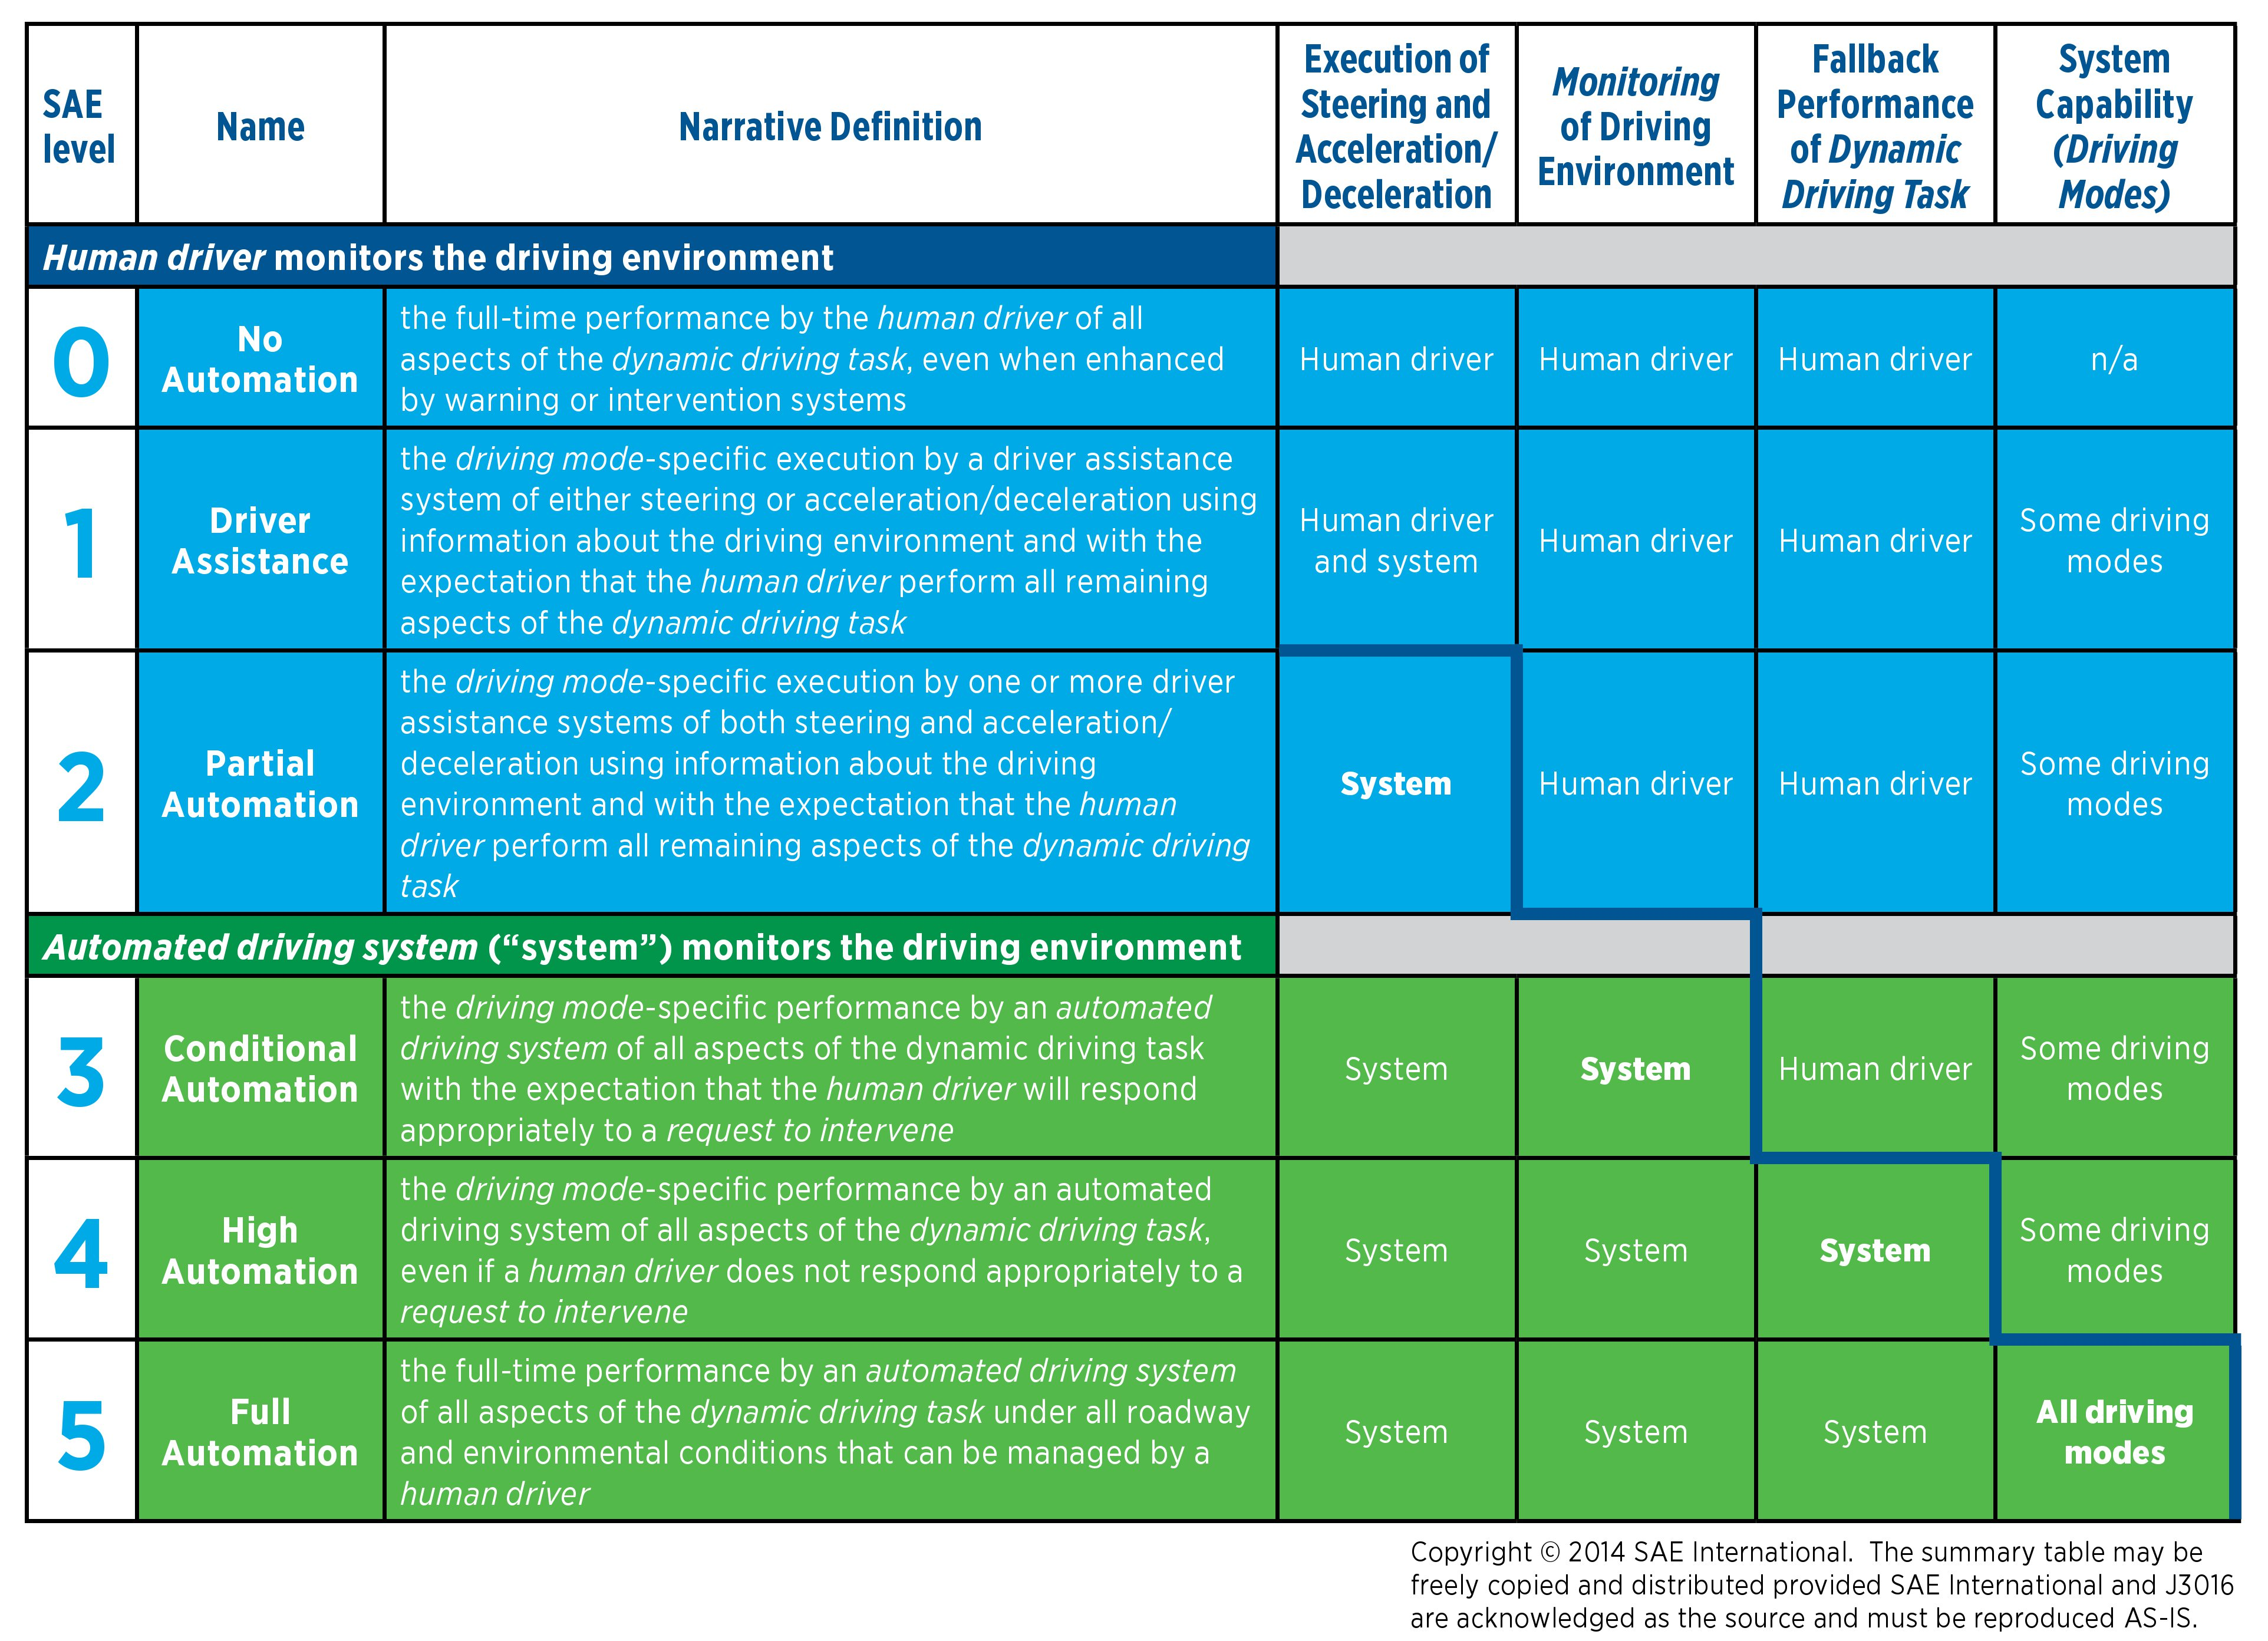
\includegraphics[scale=0.7]{level_autonomes_fahren.jpg}
\caption{Norm SAE J3016 für die Level des autonomen Fahrens, entnommen aus \cite{sae2014taxonomy}}
\label{fig_level_autonomes_fahren}
\end{figure}


% ===========================
\subsection{Entwicklung von Fahrerassistenzfunktionen}
\label{grundlagen_fahren_entwicklung}
% ===========================

\gls{fas} sind Funktionen im Kraftfahrzeug, die den Fahrer unterstützen. Diese Systeme nutzen Sensordaten, wie Radar-, Ultraschall-, oder Kameradaten, aus dem Fahrzeug um den Fahrer dann auf Basis der abgeleiteten Informationen zu unterstützen. Beispielsweise erkennt ein Spurhalteassistent wenn das Fahrzeug die Spur verlässt und kann die Fahrspur korrigieren. 

\gls{fas} werden in der Automobilindustrie mit dem V-Modell entwickelt. Das V-Modell ist ein chronologischer Entwicklungsprozess und aus der Softwareentwicklung adaptiert \cite{vmodell2005}. Das V-Modell kann in einen linken absteigenden und einen rechten aufsteigenden Ast unterteilt werden. Der linke Ast enthält die Funktionsanforderungen, die nach unten weiter detailliert und aufgeschlüsselt werden. Der rechte Ast umfasst aufsteigend Funktionstests auf dem jeweiligen Detaillierungsgrad \cite{hakuli2015virtuelle}. Das V-Modell ist schematisch in Abbildung \ref{fig_v_modell} dargestellt.

\begin{figure}[h]
\centering
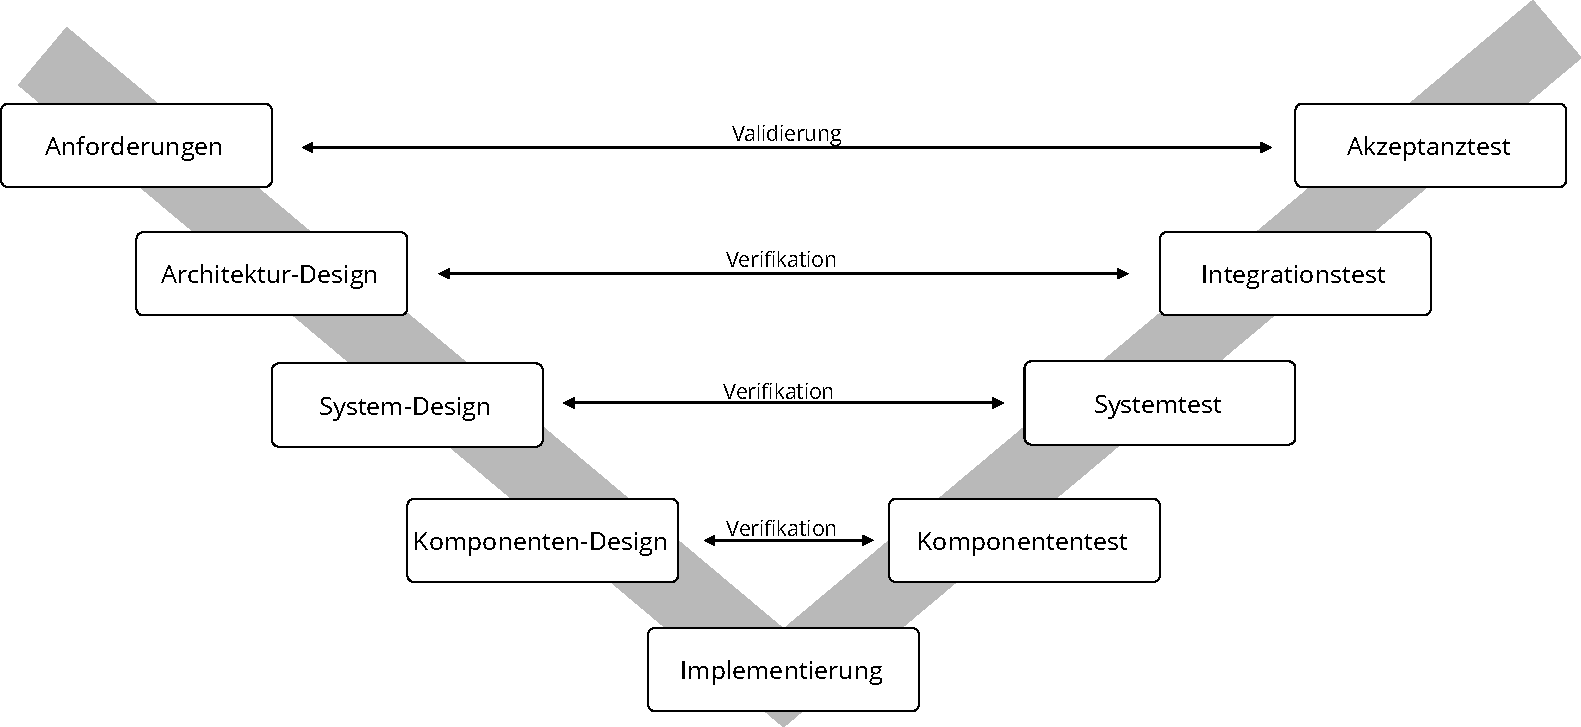
\includegraphics[scale=0.6]{v_modell.pdf}
\caption{V-Modell, adaptiert aus \cite{hakuli2015virtuelle}}
\label{fig_v_modell}
\end{figure}

Durch die steigende Komplexität werden für die Validierung und Verifikation von \gls{fas} neue Testmethoden benötigt \cite{tellmann2011hardware}. 

Diese  werden 



--- V Modell --- \cite{hakuli2015virtuelle}



Fahrerassistenzfunktionen werden funktional wei- testgehend in Software abgebildet. Daher ist es sinn- voll, das aus dem Software Engineering bekannte V-Modell[3]oder seine Weiterentwicklung „V-Mo- dell XT“ [4] als Entwicklungsprozess für Fahreras- sistenzfunktionen zu verwenden. Das V-Modell stellt grundsätzlich einen chronologischen Entwick- lungsprozess dar. Der Ablauf ist dabei nicht linear über der Zeitachse aufgetragen, sondern über die Form des Buchstabens V. Es wird dabei von einem absteigenden und einem aufsteigenden Ast gespro- chen. Der absteigende Ast enthält die Arbeitsschritte der Analyse der Aufgabenstellung. Aus der Analyse resultieren schrittweise Spezifikationen für die zu entwickelnden Komponenten. Dabei ist wesentlich, dass zunächst die Gesamtproduktanforderungen (oft auch Kundenanforderungen genannt) analysiert und danach in eine logische Architektur überführt wer- den. Im Anschluss daran folgt die Entwicklung einer technischen Architektur, die im weiteren Verlauf in Systeme und in Komponenten zerlegt und spezifi- ziert wird. Parallel zu jedem dieser Schritte entste- hen Testfallspezifikationen, die später zur Überprü- fung der Entwicklung verwendet werden. Der letzte Schritt des absteigenden Astes markiert gleichzeitig den ersten Schritt im aufsteigenden Ast. Auf ihm er- folgt die eigentliche Implementierung beziehungs- weise Entwicklung der spezifizierten Komponen- ten. Der aufsteigende Ast beinhaltet alle Test- und Integrationsschritte von der einzelnen Komponente über das Gesamtsystem bis hin zum Akzeptanztest beim Kunden. Er stellt also das Integrieren und Tes- ten im Entwicklungsprozess dar. Jeder Schritt auf dem absteigenden Ast hat eine Beziehung zu einem Schritt im aufsteigenden Ast. Dabei entspricht die Beziehung dem Verifizieren des im entsprechenden Prozessschritt erstellten Teilsystems gegenüber der zugehörigen Spezifikation. Die jeweils verwendeten Testfälle sind diejenigen, die während der Spezifikati- onsphase im absteigenden Ast entwickelt wurden. Im letzten Schritt erfolgt die Validierung, d. h. die Über- prüfung der Erfüllung aller Kundenanforderungen sowie der Akzeptanztest. . Abbildung 8.1 zeigt den generellen Entwicklungsprozess nach dem V-Modell.

-----------------------------------

Die Leitidee des virtuellen Fahrversuchs ist die möglichst realitätsgetreue Übertragung des realen Fahrversuchs in die virtuelle Welt mit dem Ziel, von den charakteristischen Stärken der Simulation in Sachen Reproduzierbarkeit, Flexibilität und Auf- wandsreduktion zu profitieren und früh im Fahrzeugentwicklungsprozess eine Test- und Bewer- tungsmöglichkeit für Spezifikationen und daraus abgeleitete Lösungen herzustellen. Die Nutzung geeigneter Simulationsverfahren ermöglicht eine effizientere Konzeption, Entwicklung und Applika- tion von Fahrzeugen und Fahrzeugkomponenten. Sie überbrücken und verkürzen die Zeit bis zur Ver- fügbarkeit von realen Fahrzeugprototypen. 

Der virtuelle Fahrversuch besteht wie sein re- ales Gegenstück aus mehreren Komponenten. Die zentrale Rolle spielt ein virtueller Fahrzeugpro- totyp, dessen Bestandteile je nach Fortschritt im Entwicklungsprozess als Modelle, Software-Code oder als Hardware integriert sind.

Während in der frühen Konzeptphase noch alle Bestandteile des Fahrversuchs virtuell sind, erfolgt im Laufe der Entwicklung durch die verschiedenen Integrationsstadien, ein schrittweiser Austausch von virtuellen gegen die zugehörigen realen Versuchsbestandteile, bis im vollständig realen Fahrversuch auf der Straße mit realem Fahrer und echten Verkehrsteilnehmern die Simulationsanteile komplett der Realität gewichen sind.

Ziel muss daher sein, entwicklungsbegleitend Teillösungen sowohl gegen die zugehörigen Spezi- fikationen zu testen als auch im gleichen Kontext im Gesamtfahrzeugkonzept auf die Erfüllung der gewünschten Eigenschaften für die Gesamtlösung überprüfen zu können. Der wirkliche Mehrwert des virtuellen Fahrversuchs besteht deshalb darin, die im realen Fahrzeug bei der Freigabe gefahrenen Manöver und die zugehörigen Bewertungskriterien durchgängig durch die in ▶ Abschn. 8.3 am Beispiel des V-Modells diskutierten Integrationsschritte bis zum Beginn der Konzeptphase zu überführen und schon dort verfügbar zu machen.

-----

For early assessment, a common approach is to set up vehicles with additional prototyping hardware and per- form real world testing. While this approach is essential to assess the look-and-feel of newly developed concepts, its drawbacks are re- duced reproducibility and high expenses to achieve a sufficient and balanced sample. To overcome these drawbacks, new flexible, realis- tic and preferably automated virtual test methods to complement real world verification and validation are especially required during early development phases \cite{bach2017reactive}.

While real world validation is indispensable, it hampers reproducibil- ity. The preliminary development phase is characterized by tight re- sources, frequent changes in design and an iterative modus operandi. Scant experience with the system properties leads to regular realign- ments and refactorings. To achieve satisfying results within an appro- priate time span, besides the RP approach further stimuli for iterative test of control systems are required. These range from test vectors modelling certain interesting waveforms and replay of recorded data to more sophisticated approaches such as Time Partition Testing (TPT) [2], which facilitates systematic testing of embedded systems with continuous behavior, or X-in-the-loop (XiL) simulation [3-5]. XiL represents a simulation based methodology for the test of embed- ded systems over all development stages of the automotive industry. The selection of the appropriate stimuli depends on the specific char- acteristics of the System under Test (SuT). As shown in Figure 1, closed-loop control systems require stimulation by methods such as XiL, RP or TPT, which offer a sufficient degree of reactiveness. Un- fortunately, these elaborate methods require significant resources for deployment and maintenance. \cite{bach2017reactive}

Reuse of naturalistic driving data recorded with RP systems offers a substantial contribution to the preliminary development of open-loop systems because sparse additional resources are needed for the provi- sion of realistic, repeatable and consistent stimuli. Closed-loop sys- tems require the simulation of a plant model for feedback and time- consuming scenario definition, leading to limited variants and real- ism. \cite{bach2017reactive}

Aktu- elle und künftige Assistenzsysteme kön- nen mit etablierten Methoden oft nur eingeschränkt oder gar nicht erprobt werden. Der derzeit vertretbare Auslöse- zeitpunkt einer automatischen Not- bremsung liegt beispielsweise in einem sehr kurzen Zeitfenster unmittelbar vor einer Kollision [3]. Deshalb erweist sich die reproduzierbare und vor allem für den Versuchsfahrer sichere Erprobung derartiger Assistenzsysteme bisher als sehr schwierig. Fahrerassistenzsysteme, die in kri- tischen Verkehrssituationen unterstüt- zen, erfordern eine Erprobung und Ab- sicherung unter nahezu realen Ver- kehrsbedingungen. Der derzeitige Stand der Technik sind Fahrsimulatoren, Ver- kehrsf lusssimulationen und Erpro- bungsfahrzeuge, die mit Ersatzobjekten wie beispielsweise Schaumstoffwürfeln kollidieren. Die derzeit verfügbaren Testwerkzeuge, einen Überblick gibt Bild 4, erfüllen die Anforderungen nach einer realistischen, reproduzierbaren, sicheren und zugleich Ressourcen scho- nenden Testumgebung allerdings nur eingeschränkt. \cite{bock2008vehicle}

Der Ansatz des Prüfaufbaus Vehicle in the Loop (VIL) von Audi liegt daher in der Kopplung des realen Testfahrzeugs mit einer virtuellen Verkehrsumge- bung, um die Vorteile beider Verfahren zu vereinen, Bild 4. \cite{bock2008vehicle}

Insbesondere die Fahrzeugentwicklung ist von vielen Innovatio- nen geprägt, die den Komfort, die Effizienz sowie die Sicherheit verbessern und optimieren sollen. Um ein globales Optimum zu erreichen, darf das System Fahrzeug nicht losgelöst von den Sys- temen Umwelt und Fahrer betrachtet werden. \cite{albers2010x}

Car-to-X-(beziehungsweise Car2X)-Technologien sorgen für die notwendige Vernetzung. Reale Fahrversuche sind aber mit einem enormen Kosten- und Zeitaufwand verbunden. Um diese durch- zuführen und Szenarien abzubilden, müssen geeignete Testgelän- de sowie eine ausreichende Anzahl an Fahrzeugen mit prototypi- schen Car2X-Systemen vorhanden sein. Zudem bieten Tests in der realen Welt oft ein geringes Maß an Reproduzierbarkeit [2]. Ak- tuell beschränken sich Simulationen im Bereich Car2X auf Appli- kations- und Protokolltests [2].\cite{albers2010x}

Das X-in-the-Loop-Framework beschreibt eine durchgängige und integrierte Entwicklungsumgebung für Antriebssysteme. Ab- geleitet wurde dieser Ansatz vom klassischen Hardware-in-the- Loop-Ansatz (HiL). Dieser bezieht sich ausschließlich auf das Tes- ten von Steuergeräten und Steuergerätefunktionen, integriert aber bereits „die Akteure“ Fahrer und Umwelt konsequent. Beim X-in- the-Loop-Framework steht das „X“ jeweils für den zu untersu- chenden Prüfling, die Unit Under Test (UUT). Diese kann eine einzelne Antriebsstrangkomponente, zum Beispiel eine Kupplung, ein Steuergeräte-Code oder ein komplettes Fahrzeug sein – jeweils real oder virtuell. Auf jedem Systemdetaillierungs-Layer (XiL-Layer) wird das Restfahrzeug simuliert. Mit dem Ziel, reali- tätsnahe Wechselwirkungen und Belastungen für die UUT zu ge- währleisten.\cite{albers2010x}

Der Simulationsfortschritt wird ge- triggert, durch diskrete Ereignisse. Je größer das betrachtete Szenario und je mehr Kommunikationsknoten oder Fahrzeugin- stanzen simuliert werden, desto mehr Ereignisse werden pro Si- mulationsschritt ausgelöst und desto höher sind folglich die An- forderungen an die Rechenleistung. Daher ist insbesondere hier die Wahl des richtigen Abstrak- tions- oder Genauigkeitsgrades wichtig. Die Technik, die dabei angewendet wird, ist das sogenannte Multi Resolution Model- ling (MRM). Dabei werden komplexe Modelle, zum Beispiel das Umwelt- oder Verkehrsmodell parameterabhängig im Detaillie- rungsgrad beziehungsweise der Performance variiert. \cite{albers2010x}

Um die funktionale Sicherheit neuer Fah- rerassistenzsysteme (FAS) abzusichern, kommen bei OEMs und Zulieferern je nach Entwicklungsphase unterschiedliche Test- und Bewertungsverfahren zum Ein- satz. Simulationsmethoden wie Model-in- the-Loop (MiL) und Software-in-the-Loop (SiL) werden vor allem in einer frühen, Hardware-in-the-Loop (HiL) in einer spä- teren Entwicklungsphase eingesetzt. Die Systeme werden in ein virtuelles Fahr- zeug integriert und im virtuellen Fahrver- such geprüft. Auf diese Weise können in sehr kurzer Zeit zahlreiche Tests unter beliebig konfigurierbaren und reprodu- zierbaren Bedingungen durchgeführt werden [1]. Diese simulativen Methoden sind allerdings kein Ersatz für den realen Fahrversuch. Auch wenn die aktuellen Modelle sehr gut sind, besteht die Unsi- cherheit, dass die Ergebnisse nicht exakt auf das reale Fahrzeugverhalten übertrag- bar sind. Darüber hinaus ist eine subjek- tive Bewertung im Fahrversuch unerläss- lich, um die Akzeptanz des Fahrers zu gewährleisten. Das Testen von FAS im klassischen Fahrversuch auf Straßen wird jedoch mit zunehmender Komplexität der Systeme immer aufwendiger. Während bei Ein- parkassistenten hauptsächlich nur ste- hende Objekte variiert werden müssen, um verschiedene Parkszenarien darzu- stellen, wird bei Systemen zur Unfall- vermeidung wie dem Notbremsassisten- ten mindestens ein potenzieller Unfall- gegner benötigt. In derzeit eingesetzten Verfahren werden hierfür sogenannte Dummy-Targets eingesetzt (zum Beispiel in [2]). Diese Ziele sind hauptsächlich für Auffahrszenarien im Längsverkehr aus- gelegt. Weitere relevante Verkehrssitua- tionen, wie etwa Querverkehr an einer Kreuzung, plötzlich einscherende Fahr- zeuge oder die Kollisionsgefahr mit Fußgängern oder Radfahrern können nur eingeschränkt beziehungsweise mit erheblichem Aufwand untersucht werden. \cite{schwab2014durchgangige}

Die neue Vehicle-in-the-Loop-Simulation (ViL) ist nach HiL und SiL eine innovative Methode, um die Komplexität bei der funktionalen Absicherung von Fahrerassistenzsystemen beherrschbar zu machen und gleichzeitig den Testaufwand zu reduzieren. Diese Methode kombiniert die Vorteile des Fahrversuchs und der Simulation, indem ein reales Fahrzeug in eine virtuelle Verkehrsumgebung eingebunden wird. \cite{schwab2014durchgangige}

Dieses Testkonzept bietet folgende Vorteile:
: reale Fahrdynamik
: weniger materieller Aufwand als im rein realen Fahrversuch
: reproduzierbare Testbedingungen
: beliebig konfigurierbare Szenarien. 

Weitere Anwendungsfelder für ViL sind unter anderem das Testen von Spur- wechselassistenten, Notbremsassistenten mit und ohne Fußgänger- beziehungs- weise Radfahrererkennung, Ausweich- assistenten sowie die Untersuchung kom- plexer, autonomer Fahrfunktionen im virtuell fließenden Verkehr. \cite{schwab2014durchgangige}



% ===========================
\subsection{Klassifizierung von Fahrszenarien}
\label{grundlagen_fahren_szenarien}
% ===========================

- Terminologie, Unterschiedung Szene, Szenario, ...
- Tabelle + Erklärung

Duis autem vel eum iriure dolor in hendrerit in vulputate velit esse molestie consequat, vel illum dolore eu feugiat nulla facilisis at vero eros et accumsan et iusto odio dignissim qui blandit praesent luptatum zzril delenit augue duis dolore te feugait nulla facilisi.   


% ===========================
\section{Künstliche Neuronale Netze}
\label{grundlagen_nn}
% ===========================

Duis autem vel eum iriure dolor in hendrerit in vulputate velit esse molestie consequat, vel illum dolore eu feugiat nulla facilisis.


% ===========================
\subsection{Maschinelles Lernen}
\label{grundlagen_nn_ml}
% ===========================

Duis autem vel eum iriure dolor in hendrerit in vulputate velit esse molestie consequat, vel illum dolore eu feugiat nulla facilisis at vero eros et accumsan et iusto odio dignissim qui blandit praesent luptatum zzril delenit augue duis dolore te feugait nulla facilisi. 


% ===========================
\subsection{Convolutional Neural Network}
\label{grundlagen_nn_cnn}
% ===========================


\begin{table}[h]
\centering
\begin{tabular}{l | l | l}
A & B & C \\
\hline
1 & 2 & 3 \\
4 & 5 & 6
\end{tabular}
\caption{very basic table}
\label{tab:abc}
\end{table}


% ===========================
\subsection{Recurrent Neural Network}
\label{grundlagen_nn_rnn}
% ===========================

Lorem ipsum dolor sit amet, consectetuer adipiscing elit, sed diam nonummy nibh euismod tincidunt ut laoreet dolore magna aliquam erat volutpat \cite{latexcompanion}. 


% ===========================
\subsection{Training mit synthetischen Daten}
\label{grundlagen_nn_synthetisch}
% ===========================

Lorem ipsum dolor sit amet, consectetuer adipiscing elit, sed diam nonummy nibh euismod tincidunt ut laoreet dolore magna aliquam erat volutpat \cite{latexcompanion}. 


